\section{Sisätilapaikannuksen sovellukset}
Tässä luvussa käsitellään sisätilapaikannuksen sovelluksia. Alkuun käsitellään sovelluksia yleisesti ja sen jälkeen siirrämme painopisteen kaupan alan sovelluksiin. Lopuksi teemme katsauksen tulevaisuuteen sisätilapaikannuksen sovelluksien osalta ja esitämme arvioita minkä tyyppisellä sovelluksella tehdään läpimurto ja sisätilapaikannuksen sovellukset alkavat yleistyä.

\subsection{Sovellukset yleisesti}
Sisätilapaikannuksella on monia sovelluksia ja monet nykyiset sovellukset ja järjestelmät hyötyisivät mahdollisuudesta tietää itsensä tai käyttäjänsä sijainti. Yleisesti sisätilapaikannus yhdistetään vain sisätila navigointiin mutta sisätilapaikannus tarjoaa paljon muitakin mahdollisuuksia. Seuraavassa esimerkkejä sisätilapaikannuksen sovelluksista. 

\begin{description}
\item[Varastot]\hfill \\
Tavaroiden sijainnin ja lukumäärän selvittäminen. Tällä tavalla voidaan pitää pienempiä varastoja kun tidetään varaston saldot tarkalleen reaaliaikaisest, eikä inventaarioita tarvitse tehdä käsin, mikä säästää aikaa ja täten rahaai. Voidaan käyttää myös optimaalisen reitin löytämiseen useaa tavaraa haettaessa. Varaston automatisointi on myös mahdollista sisätilapaikannuksen avulla.
\item[Sairaalat]\hfill \\
Äkilllisissä tilanteissa lääkärin tai muun sairaala henkilökunnan löytäminen nopeasti\cite{ibeacon} tai automaattisesti lähimmän hoitajan hälyttäminen paikalle. Myös potilaiden paikannus on tärkeä sovellus varsinkin vakavasti sairaiden potilaiden kohdalla.
\item[Robotit]\hfill \\
Navigointi kyky sisätiloissa. Lisää työturvallisuutta teollisuuden koneiden läheisyydessä ja parantaa sisätiloissa liikkuvien koneiden toimintakykyä.\cite{lips}
\item[Kampus]\hfill \\
Luentosalin löytäminen, hyödyllinen etenkin uusille opiskelijoille ja vieraileville luennoitsijoille \cite{campus}.
\item[Museo]\hfill \\
Edessä olevan taideteoksen esittely esimerkiksi puhelimeen. Mahdollisesti käyttäjää kiinnostavien teoksien luokse ohjaaminen. Museolle arvokasta tietoa asiakkaiden kulkureitestä palveluiden parantamiseksi.
\item[Parkkihallit]\hfill \\
Vapaan paikan löytäminen tai oman auton löytäminen\cite{lips}.
\end{description}

Edellä mainittujen sovelluksien lisäksi on olemassa tietenkin monia muitakin sovelluksia. Tässä työssä tarkastelemme tarkemmin kaupan alan sovelluksia. Niitä käsittelemme seuraavassa alaluvussa.

\subsection{Kaupan alan sovellukset}
Sisätilapaikannuksen sovellukset kaupan alalla voidaan jakaa kolmeen käyttötarkoituksen perusteella: kuluttajasovellukset,sovellukset kaupalle ja markkinoinin ja mainonnan sovellukset.

Kuluttajasovelluksilla tarkoitetaan sovelluksia, jotka ovat suunniteltu palvelemaan kuluttajan tarpeita ja toiveita. Tälläisiä sovelluksia ovat esimerkiksi navigointi sovellukset. Nämä ovat hyödyllisiä varsinkin suurissa kaupoissa ja ostoskeskuksissa. Kauppakeskus navigaattori sovelluksen avulla käyttäjä löytää etsimänsä kaupan hakemalla tuotteen, tuoteryhmän, palvelun tai jonkin muun kiinnostavan kohteen nimen avulla. Navigaattori voi myös viedä tarkalleen oikean hyllyn kohdalle josta kyseinen tuote löytyy. Näin myös on mahdollista antaa navigaattorille ostoslista ja navigaattori laskee helpoimman reitin kaikkien tuotteiden löytämiseksi. Helpoin reitti ei toisaalta ole kaupan kannalta välttämättä paras reitti, sillä silloin heräteostokset jäävät vähemmälle, kun kaupassa ei tarvitse niin paljon kiertellä ja etsiä. Tämän takia kaupat itse tuskin tarjoavat tämän tyyppisiä sovelluksia, vaan ne tulevat joltain kolmannelta osapuolelta. Kaupat voisivat toki määrittää parhaan reitin siten, että se kulkee mahdollisimman monen tarjous tuotteen ohi, jolloin myös heräteostoksia tapahtuu todennäköisesti enemmän. Näiden tyyliset navigointi sovellukset ovat hyödyllisä eritysesti suurissa ostoskeskuksissa ja sellaisissa kaupoissa jotka eivät ole tuttuja käyttäjälle, etenkin ulkomailla joissa kyltit eivät aina helpota tavaroiden löytymistä.

Toinen kuluttajasovellus, joka toimii parhaiten vastakkaisessa tilanteessa kuin edellinen liittyy ns. sosiaalisiin sovelluksiin. Edellinen esitelty navigaattori sovellus on hyödyllisimmillään oudoissa paikoissa, joissa ohjaus voi helpottaa hyvinkin paljon asioimista. Tässä esitelty sovellus  on taas parhaimmillaan omalla kotiseudulla tutussa ympäristössä. Sisätilapaikannus mahdollistaa sovelluksen jossa käyttäjä voi katsoa ketkä hänen ystävistään ovat hänen kanssaan samaan aikaan paikalla esimerkiksi samassa ostoskeskuksessa ja sovellus voi ohjata heidän luokseen.  Tällä sovelluksella on myös hyötyä markkinoinnissa ja mainonnassa, josta lisää luvussa 4. Tämänlainen sovellus voi helpottaa myös vanhempien elämää, kun voivat tarkistaa mihin heidän hetki sitten vielä vieressä ollut lapsensa on karannut. Tämänlaisissa tilanteissa sovellus on hyödyllisimmillään etenkin kaikista ruuhkaisimpina aikoina.

Kolmas sovellus sisätilapaikannuksen kaupan alan kuluttajasovelluksissa on nopeimman kassajonon valitseminen ja arvioidun jonotus ajan määrittäminen. Tämä sovellus vaatii jo hieman enemmän infrastruktuuria kuin edellä mainitut joissa riittää pelkkä puhelin. Tämän sovelluksen voisi toteuttaa siten että, ostoskärryissä ja koreissa voisi olla RFID lukijat jotka lukevat tuotteissa olevia RFID tunnisteita ja määrittää siten kuinka monta tuotetta asiakkaalla on, toinen tapa olisi viivakoodin lukija jolle tuotetta näytetään aina kun se laitetaan kärryyn. Kumpikin on toki hieman haasteellinen varsinkin ostoskorien osalta joissa ei voi olla kovin suurta virtalähdettä siten että korista ei tule painava. Kolmas tapa voisi olla tutkia asiakkaiden(kärryjen tai korien) liikettä. Asiakkaan pysähtyesä hyllyn kohdalla ja hyllystä tuotteen kadotessa voidaan olettaa, että asiakas on ottanut sen. Tässä tavassa on myös omat heikkoutensa. Jos vierekkäin on monta asiakasta on vaikea arvata mille asiakkaalle mikäkin tuote on mennyt tai jos asiakas jättääkin tuotteen jonnekkin sille kuulumattomalle paikalle tuoteiden määrän arviointi on vaikeaa. Tällä tavalla voidaan kuitenkin saada arvio tuotteiden määrästä ja se on käytännöllisempi toteuttaa, kuin edellä mainitut tavat. Kun tiedossa on asiakkailla olevat tuotteet ja heidän sijaintinsa voidaan arvioida kuinka kauan niiden lastaaminen kassalle, maksaminen ja purku kestää.
  
Edellä mainitut sovellukset ovat olleet kuluttajasovelluksia. Seuraavaksi käsitellään sovelluksia joita käytetään kaupoissa mittaamaan asiakkaiden käyttäytymistä ja siten parantaa kaupan järjestelyitä vastaamaan ja muokkaamaan tätä käytöstä. Kaupat ovat nykyään kiinnostuneita siitä kuinka asiakkaat liikkuvat kaupan tiloissa, eikä vain siitä mitä he ostavat\cite{heat}. Sisätilapaikannus tarjoaa tämän tiedon keräämiseksi sopivia teknologioita. Sisätilapaikannuksella voidaan seurata asiakkaiden liikkeitä kaupassa, ja näistä liikkeistä voidaan muodostaa lämpökartta. Lämpökartoissa alue on värjätty sitä punaisemmaksi, mitä enemmän sillä kohdalla on ollut liikettä. Siniset alueet ovat alueita joissa ei ole käynyt juuri kukaan. 
\begin{figure}[htpb]
    \centering
    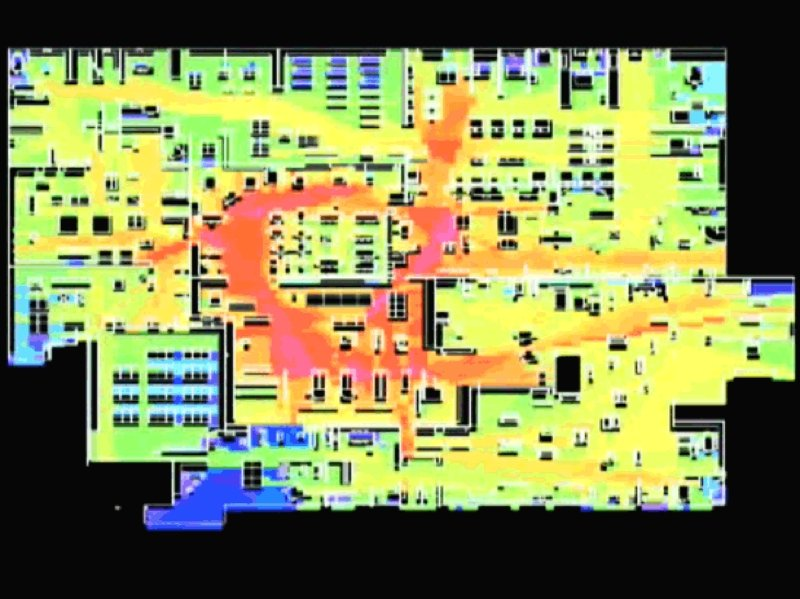
\includegraphics[width=0.6\textwidth]{ikeaheatmap.png}
    \caption{Lämpökartta Ikea tavaratalossa käyneiden asiakkaiden kulkureiteistä\cite{ikea}}
    \label{ikea}
\end{figure}
Näin lämpökartoista nähdään missä asiakkaat liikkuvat eniten tutkimalla kartan väritystä. Tämän tiedon pohjalta kaupat voivat järjestellä suositut ja epäsuositut ja halvat ja kalliit tuotteet optimaalisesti\cite{heat}.
Kuvassa \ref{ikea} nähdään, että käytännössä kaikki Ikeassa käyneet kulkivat pääkäytävää, joten sen varrelle on hyvä sijoittaa esimerkiksi sopivia tavaroita heräteostoksiksi.
Lämpökartoista voidaan myös selvittää mitkä tuotteet ovat olleet kiinnostavia, mutta niitä ei ole kuitenkaan ostettu. Tämä onnistuu siten, että tutkitaan tuotteen sijaintia lämpökartalla ja samalla tutkitaan tuotteen myyntiä. Tuotteet jotka ovat lämpökartalla punaisella alueella mutta niiden myynti on kuitenkin huonoa, saattavat olla liian kalliita asiakkaiden näkökulmasta ja niiden hinnoittelua voisi olla syytä harkita uudelleen.

%mainonta
Kolmas sisätilapaikannuksen kaupan alan sovellusten ryhmä on markkinointi ja mainonta. Tätä aihetta käsitellään seuraavassa luvussa.

\subsection{Yhteenveto ja tulevaisuus}

Sisätilapaikannuksen sovelluksia löytyy lähes kaikilta elämän osa-alueilta. Osa sovelluksista perustuu pelkästään sisätilapaikannukseen, kuten navigointi sovellukset, ja osassa sovelluksista sisätilapaikannuksella voidaan luoda lisäarvoa jo olemassa oleviin sovelluksiin, esimerkiksi varasto sovellukset.

%killeri appi
%selvästi vaikeampi arvioida suuren vaihtoehtojen määrän takia.



